\documentclass[graphics]{beamer}

\usepackage{graphicx}
\usepackage{verbatim}
\usepackage{wrapfig}
\useoutertheme{shadow}
%\usecolortheme{orchid}
\usecolortheme{seahorse}


% math commands
\newcommand{\be}{\begin{eqnarray}}
\newcommand{\ee}{\end{eqnarray}}
\newcommand{\beq}{\begin{equation}}
\newcommand{\eeq}{\end{equation}}
\def\simless{\mathbin{\lower 3pt\hbox
      {$\rlap{\raise 5pt\hbox{$\char'074$}}\mathchar"7218$}}}
\def\simgreat{\mathbin{\lower 3pt\hbox
      {$\rlap{\raise 5pt\hbox{$\char'076$}}\mathchar"7218$}}} %> or of order

% variables

\def\toonscale{0.45}
\def\mboxy#1{\mbox{\small #1}}


\begin{comment}
\AtBeginSection[]{
  \frame{
    \frametitle{Outline}
    \tableofcontents[currentsection]
  }
}
\end{comment}

\title{Options for the Universe
}
\subtitle{}
\author[U. Pen]{\textcolor{red}{
Ue-Li Pen
}
\\[8mm] 
ASIAA, CITA
}
\date{Feb 27, 2024}


\begin{document}

\frame{
\titlepage
}

%\section*{Introduction}

\begin{comment}
  \subsection{Outline}

  \frame{
    \frametitle{Outline}
    \tableofcontents
  }
\end{comment}


\frame{
\frametitle{Gravitational Waves}
\begin{itemize}
\item Nobel Prize 1993, 2017  intrinsically highly polarized
\end{itemize}
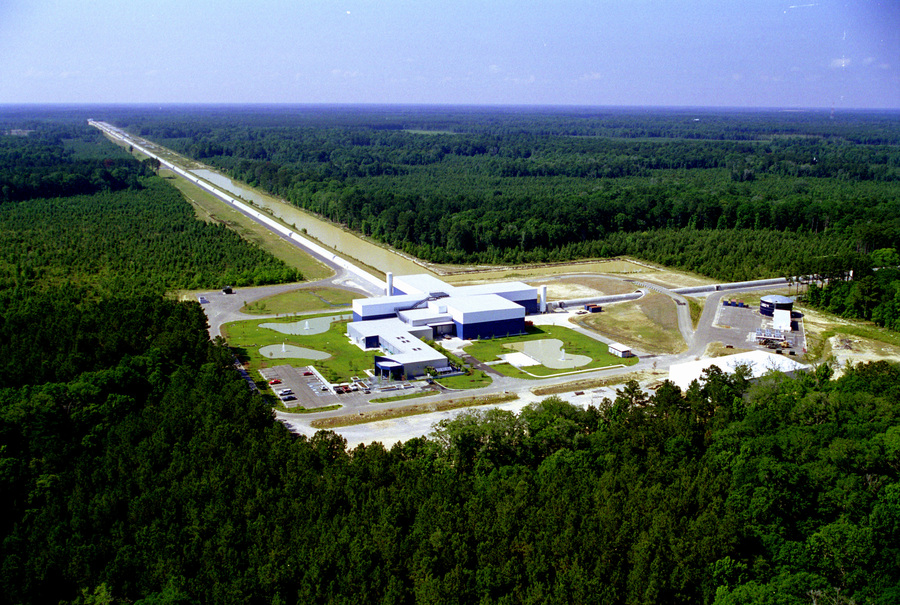
\includegraphics[width=2.7in]{Figures/ligo-livingston-aerial-02.jpg} \
\ LIGO Livingston\\
\includegraphics[width=4.5in]{Figures/LIGO_blackhole.jpg}
}

\frame{
\frametitle{Signal}
\begin{itemize}
\item measure difference of arm lengths 4 km$(1\pm h)$
\end{itemize}
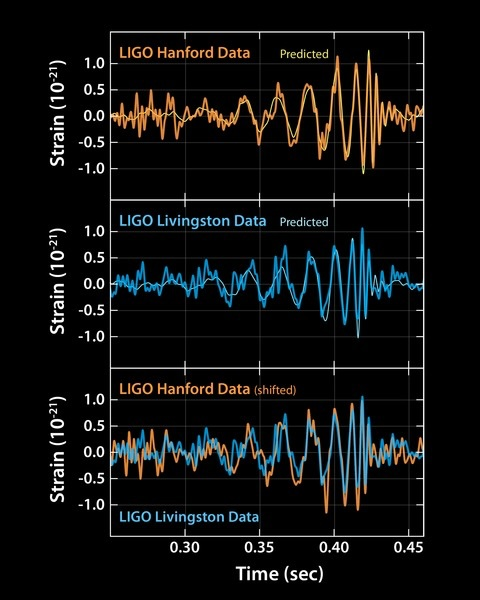
\includegraphics[width=2.3in]{Figures/ligo150914.jpg} \ \ \ 150914
}


\frame{
\frametitle{GR}
\begin{itemize}
\item $ds^2=-(1-2\phi)dt^2+[(1+2\phi)\delta_{ij}+h_{ij}] dx^i dx^j$
\item strain $h=h_L+h_R$
\item $h\sim 1$ at horizon $r_g$ (km)
\item $h \propto r_g/r, r\sim 10^{21}$km
\item strain at earth $h\sim 10^{-21}$
\item intrinsically highly polarized
\item near future polarization detection
\item polarized (chiral) background? (Masui++Pen, 2017, PRL 118, 1301)
\item neutrinos are chiral!
\end{itemize}
}



\frame{
\frametitle{Polarization}
\begin{itemize}
\item left vs right
\item needs detectors rotated by 45 degrees: $h_+,h_\times$
\item possible with LIGO-Virgo-KAGRA-IndIGO
\end{itemize}
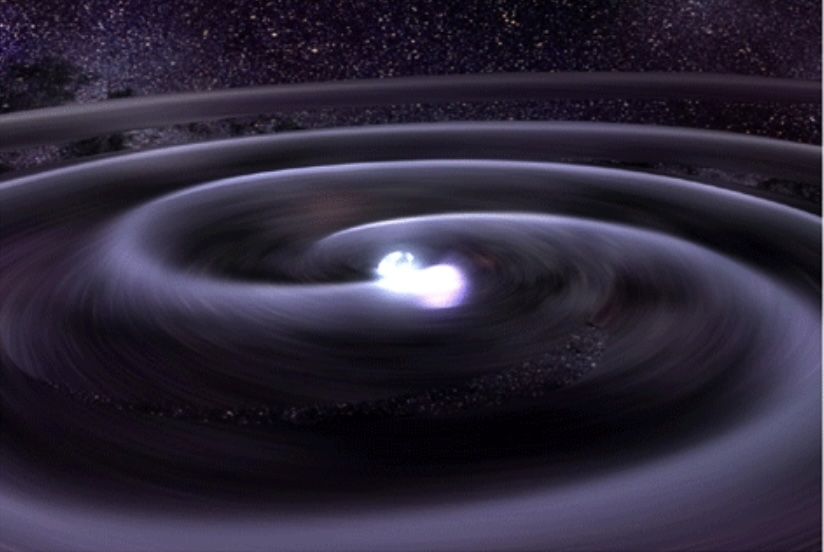
\includegraphics[width=2.1in]{Figures/spiral.jpg}
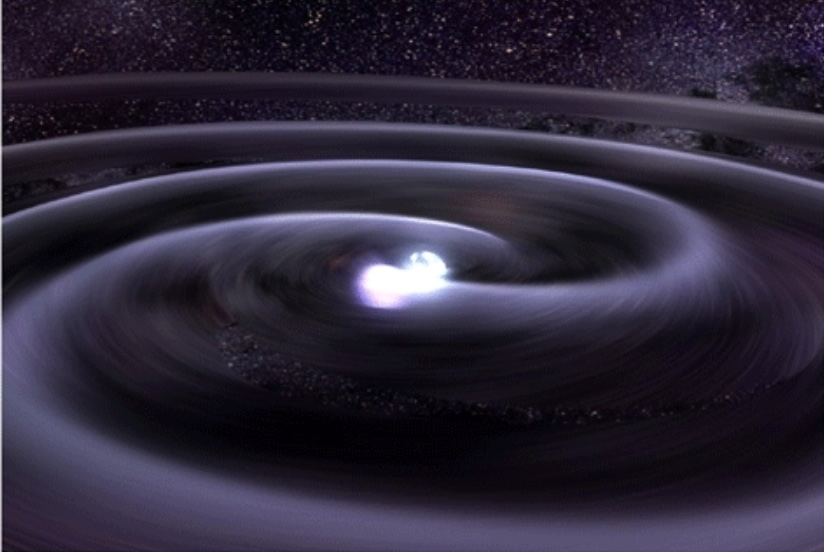
\includegraphics[width=2.1in]{Figures/spiralflip.jpg}
}

\frame{
    \frametitle{Cosmological Effects}
    \begin{itemize}
    \item redshift: wavelength gets longer, amplitude weaker
    \item small effect for current signals ($z\ll 1$)
    \item in contracting universe (looking back in time), signal gets
      bigger
    \item does it 'diverge'? (Kodwani ++ ULP, 2019a,b)
     \end{itemize}
  }


\frame{
    \frametitle{Cosmological EoM}
    \begin{itemize}
    \item $ ds^2 = a^2(\tau) \left( -d \tau^2 + (\delta_{ij} + h_{ij})
        dx^i dx^j \right)$
    \item $ h^{\text{rad}}_k(k\tau) = A^{\text{rad}}_k j_0(k\tau) + B^{\text{rad}}_k y_0(k\tau)$
    \item $j_0(u) = \frac{\sin{u}}{u}, \hspace{3mm} y_0(u) = -\frac{\cos{u}}{u}$
     \end{itemize}
  }



\frame{
    \frametitle{Cosmological Perturbations}
    \begin{itemize}
    \item cosmological GW waves not yet detected.  Major goal of
      next experiments (CMB-S4, Ali, etc)
        \item traditionally thought of as an initial value problem (IVP)
        \item challenges in specifying IVP at a singularity
        \item blinded by inflationary calculations
        \item bounce paradigm allows broader analysis
     \end{itemize}

  }



\frame{
    \frametitle{Analogy: Milne Universe decaying mode}
   \begin{itemize}
   \item Milne: $\Omega=0$ hyperbolic reslicing of Minkowski
\item $ds^2=-d\tau^2+\tau^2(\frac{d\chi^2}{1+\chi^2}+\chi^2 d\Omega)$
        \item Gauge transform from Minkowski
        \item $r=\tau\chi$, $t=\tau \sqrt{1+\chi^2}$
     \end{itemize}

  }

  \frame{
    \frametitle{Decaying modes}
\begin{itemize}
\item test fluid in Milne (empty) space:
\item has decaying modes
\item if viewed in crunch, decaying mode becomes growing mode!
\item but by construction, no gravity at play.
\end{itemize}
}


\frame{
  \frametitle{Combined constraint}
  \includegraphics[width=4in]{Figures/delens_renorm.pdf}

  \caption{Delensed B+E+T (1910.01416)}
}

  \frame{
    \frametitle{Other decaying modes?}
\begin{itemize}
\item scalar: similar effect (Kodwani++ULP 2017)
\item vector: appears uniquely absent
\end{itemize}
}

\frame{
  \frametitle{Scalar modes}
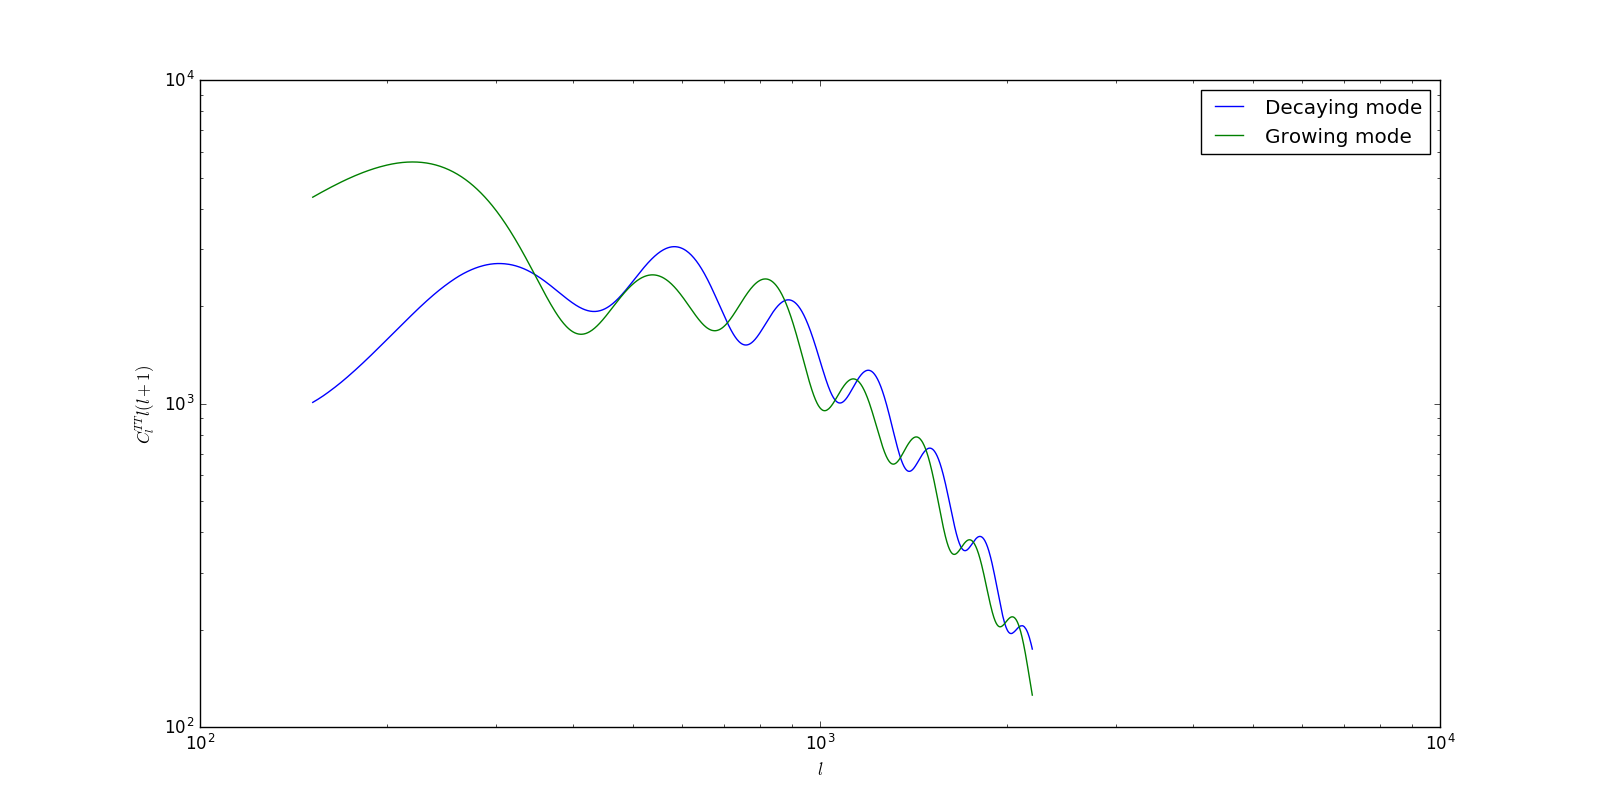
\includegraphics[width=5.1in]{Figures/TT_decaygrow_normeye_l150.png}
Similar analysis for two scalar modes
(Kodwani++ULP 2017a)
}



\frame{
\vspace{-0.5in}
    \frametitle{Conclusions}
    \begin{itemize}
      \item General Relativity has long history of confusion over
        gauge modes
      \item singular of metric not useful for physical effect!
      \item Milne universe a helpful analogy
      \item current cosmological model a combination of data
        constraints and human bias
      \item minimal inflation consistent with bias
      \item opportunities for studying irregular and chiral modes!
      \item non-linear effects?
      \item parity symmetry, regular mode are bias, unconstrained by data
     \end{itemize}
  }


\end{document}
